\documentclass[12pt]{article}
\usepackage[francais]{babel}
\usepackage[utf8]{inputenc}
\usepackage{graphicx}
\usepackage{amsmath}
\usepackage{amsfonts}
\usepackage{amssymb}




\addtolength{\hoffset}{-1cm}
\addtolength{\textwidth}{2cm} 
\addtolength{\voffset}{-1cm}
\addtolength{\textheight}{2cm} 

\begin{document}

\begin{titlepage}
\begin{center}

\hfill
\vfill
\bigskip
\huge{ 
\includegraphics[width=60,height=50]{logo.png} 

\includegraphics[width=80,height=50]{lh.png} \\
U.F.R Sciences et Techniques \\
M2 MATIS  \\
 Rapport de stage \\  \\ \\ \\ \\
 } 
\vfill
\bigskip 
\Huge 
\bigskip %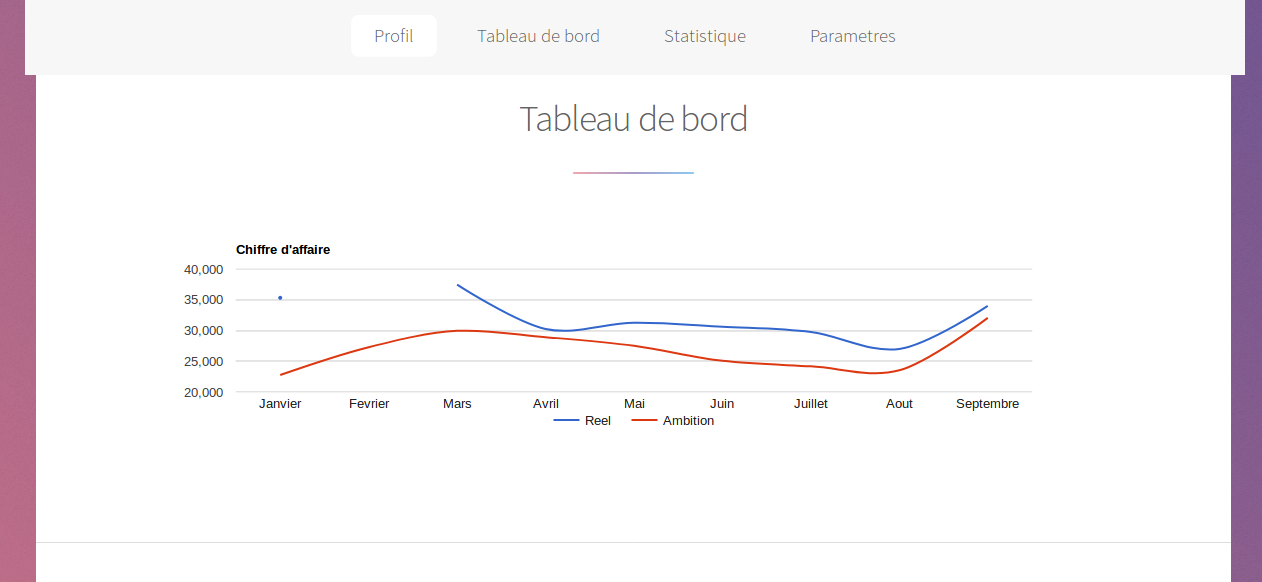
\includegraphics[width=150,height=120]{pg2.png}} 
\\ \\
\textbf{ Développement d'un site web de gestion des entreprises sous Symfony 3 } \par 
\vfill

\Large \begin{flushleft}
 Réalisé par:\\ sidi Maouloud \par
\end{flushleft}
		 
		  \begin{flushright}
		                    sous la direction de:\\  M. ould Maouloud
		                   \end{flushright}



		 
\vfill
\Large Université du Havre \par \Large VMP Consulting		
		\bigskip 
\bigskip

\Large
Juillet-Novembre 2017
\end{center}
\end{titlepage}

\section*{Remerciements}


J’adresse mes remerciements à  M. sidi ould MAOULOUD, de m’avoir accueillie pour faire mon
stage au sein de son entreprise, ainsi pour son aide et  ses  remarques pertinentes.  \\ \\
J’aimerais aussi remercier M. Laurent Amanton  et tous mes enseignants de l’université du havre
qui m’ont accompagné 
au cours de l'année université 2016/2017.\\ \\

Enfin  Je tiens á transmettre ma gratitude et mon affection à mes
parents  pour leur patience et leur soutien.\\ \\


\newpage

\section*{Résumé}
\textbf{VMP-CONSULTING}  est un bureau spécialisé dans le contrôle de gestion pour les TPE/TPI, les PME/PMI et les collectivités territoriales. Il  accompagne et conseille les entreprises pour aller vers l'efficacité et l'efficience dans l'utilisation de leurs ressources afin d'atteindre leurs objectifs.\\
Pour mieux servir ses clients, \textbf{VMP-CONSULTING}  veut avoir un portail web pour 
mettre en œuvre un espace de travail unique pour les clients, 
 proposer aux clients un accès privilégié et personnalisé à divers services en
ligne, et 
développer des outils qui permettent aux clients de réagir avec les contenus du
portail.\\
L'objectif de ce stage est de réaliser ce site web.


\section*{Abstract}
Whatever the activity, today all companies are confronted with increased competitive pressure, technological changes ... To enable managers and operational staff to devote themselves entirely to their core business, support in managing The company is a necessity not to say an obligation. In this area, not all businesses are housed in the same category, particularly small businesses and small businesses. The lack of management tools is mainly linked to a problem of means although sometimes it can be a problem of awareness of the utility and the benefit brought by these tools.\\
\textbf{VMP-CONSULTING}  is an office specializing in management control for small and medium-sized enterprises (SMEs), SMEs and local authorities. He accompanies them and advises them to move towards efficiency and efficiency in the use of their resources in order to achieve their objectives.\\
To better serve its customers, \textbf{VMP-CONSULTING}  wants to have a web portal for
implement a unique workspace for customers,
 offer customers privileged and personalized access to various services in
line, and
develop tools that enable clients to react with the contents of the
portal.\\
The objective of this traineeship is to realize this website

\newpage
\renewcommand{\contentsname}{Sommaire}
\tableofcontents
\newpage



\section{Introduction}

\subsection{Préambule}

Quelle que soit l’activité, aujourd’hui toutes les entreprises sont confrontées à une pression concurrentielle accrue, aux évolutions technologiques...Pour permettre aux managers et aux opérationnels de se consacrer entièrement à leur cœur de métier, un accompagnement dans la gestion de l'entreprise est une nécessité pour ne pas dire une obligation. Dans ce domaine là, les entreprises ne sont pas toutes logées à la même enseigne, en particulier les TPE(Trés Petite Entreprise) et certaines PME(Petite Moyenne Entreprise). Le manque d’outils de gestion est principalement lié à un problème de moyens même si parfois il peut s’agir d’un problème de sensibilisation à l’utilité et le bénéfice apporté par ces outils.\\ \\

Le Contrôle de gestion est le garant de la bonne santé de la structure en s'assurant que les ressources sont employées efficacement.\\ 
Il intervient également pour fournir les outils qui vont servir aux décideurs pour suivre l'impact de leurs actions. Celles-ci résultant de décisions de portées stratégiques et tactiques.\\

Dans de nombreuses entreprises, il est en charge du management du système de pilotage avec la prise en charge des tableaux de bord destinés à la direction et aux responsables opérationnels.\\ \\

Ainsi la rapidité de réaction est, plus que jamais, un facteur essentiel de l’aptitude 
d’une  entreprise  à faire  face  à la  concurrence.\\ \\

 


\subsection{VMP Consulting}


VMP-Consulting est un bureau spécialisé dans le contrôle de gestion pour les TPE/TPI(trés petite entreprise), les PME/PMI(petite moyenne entreprise) et les collectivités territoriales. Il  accompagne et  conseille  les entreprises pour aller vers l'efficacité et l'efficience dans l'utilisation de leurs ressources afin d'atteindre leurs objectifs.\\ \\


VMP Consulting accompagne les PME/PMI et TPE/TPI pour la maîtrise de leur performance, avec ses solutions, pour atteindre les objectifs de :
\begin{itemize}

\item Maîtriser les coûts.

\item Optimiser les performances.

\item Une transparence sur la gestion des ressources de  l'entreprise.

\item Le développement de la réactivité dans la prise de décisions stratégiques.
\end{itemize}
\\ \\ 


Parmi ses services :
\begin{itemize}

\item \textbf{Pilotage d'entreprise: } Des conseils en gestion et pilotage d'entreprise permettent aux managers et aux opérationnels de disposer d’un système de contrôle de la performance et d’aide à la décision.


\item \textbf{Audi: } Un audit qui permet de donner une situation précise de l'entreprise, un
diagnostic qui  permettra de développer les activités, gérer efficacement les risques et prendre les bonnes décisions stratégiques dans les meilleures conditions.


\item \textbf{Système d'information : }  Assistance à la maîtrise d’ouvrage et accompagnement du changement,
 Coordination et gestion de projets, 
 Elaboration des cahiers de charges et des spécifications fonctionnelles, 

 Audit de systèmes d’informations, et

Elaboration d’outils spécifiques.


\item \textbf{Formations: } VMP apporte toute son expérience pour des formations qui permettrons de maîtriser tous les outils nécessaires à la bonne marche de l'entreprise.
\end{itemize}
\\ \\ 



Le dirigéant de la startup a une expérience de plus de 20 ans dans divers secteurs d'activités et dans plusieurs types de structures (PME - Multinationales - Organismes d'Etat), et en 2016 il a lancé       \textbf{VMP-CONSULTING} .



 \subsection{Problématique}

L’enjeu pour une entreprise aujourd'hui est d’adresser une communication ciblée en proposant un contenu pertinent au client, par exemple, mettre en avant tous ses produits et offres complémentaires permet d’informer ses clients et de déclencher de nouvelles ventes. \\ 
Pour un bureau d’études, comme \textbf{VMP-CONSULTING}  spécialisé dans la maîtrise des performances des entreprises, la mise en place d'un site internet,  permet de  Capitaliser les informations et les savoir-faire,
    simplifier la recherche d’informations,
    centraliser l’ensemble des données en un seul accès et
    fédérer les collaborateurs et les utilisateurs autour de l’entreprise.
\\ \\

Un portail web est une plate-forme collaborative dont la fonction première est de proposer aux internautes des ressources et services numériques en rapport avec un thème, un domaine d’intérêt et dédié à chaque communauté particulière (les collaborateurs, les partenaires, les clients ou encore les fournisseurs …).\footnote{www.everwin.fr}  \\
Il s’agit d’un espace de travail unique, personnalisé et sécurisé avec des droits d’accès par utilisateur.\\ \\


Ce future site web de \textbf{VMP-CONSULTING}, dédié aux entreprises clientes, sera un outil important
 de gestion des entreprises en ligne et qui pourra répondre à certains besoins du bureau d'études:
\begin{itemize}

\item  Dynamiser la collaboration avec les interlocuteurs internes et externes
 \item   Permettre la transmission des connaissances pour une organisation plus productive et performante
 \item     Améliorer le suivi des prestations réalisées par les consultants techniques : suivre en temps réel les interventions chez les clients afin d’accélérer la prise en charge directement depuis le terrain, disposer d’indicateurs et de statistiques pour détecter les problèmes récurrents.
 
 \item   Renforcer  l'offre auprès des clients, les fidéliser avec de nouveaux services
 \item   Optimiser certaines tâches back-office : accès aux données et à l’historique des  clients, avancement des taches, ...
\item    Répondre à de nouvelles exigences et garder une longueur d’avance.

\end{itemize}

\\ \\

A l'aide d'un portail web  \textbf{VMP-CONSULTING} pourra atteindre ses objectifs :

\begin{itemize}

\item Améliorer la productivité des services de l'entreprise.
\item Fidéliser les clients.
\item Se différencier par rapport à la concurrence en proposant un panel de services à
valeur ajoutée.
\item Conquérir de nouveaux clients.
\end{itemize}



\subsection{Environnement et Missions}

La mission était la prise en charge totale du projet de mise en place d'un portail internet,
j'avais en charge toutes les phases du projet de la rédaction de cahier de charges jusqu'à la phase de test en 
passant par les spécifications personnelles, les choix techniques, la modélisation et conception.\\
Parmi les difficultés rencontrées est le manque de ressources en développement de VMP-CONSUTLING ce qui a nécessité pour moi 
de passer plus de temps dans la recherche des outils de développement.
Mes missions en tant que le seul développeur du projet sont : \\
\begin{itemize}
\item Rédaction  du cahier des charges.
\item Analyse des données et proposition des solutions.
\item Conception  du site internet .  
\item Modélisation de la base de données.
\item Développement et Implémentation .
\item test et déploiement du portail web.
\end{itemize}
\\ \\
On parle souvent de cycles de vie, qui ont pour but d’organiser ces étapes de différentes manières en fonction d’un certain nombre de critères relatifs au projet de développement.\\
Le cycle de vie en cascade a été utilisé, puisque 
les besoins ou exigences n’évolueront pas en cours de projet, 
tous les besoins ont été fixés et détaillés dans le cahier des charges.
En pratique, une étape ne démarre que si la précédente ait été validée par le client.

\\
\begin{center}
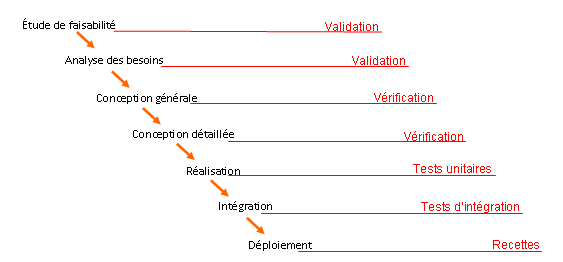
\includegraphics[width=250,height=250]{p.png}}
 
\end{center}
\\ \\



\newpage

\section{ Cahier des charges et spécifications fonctionnels}

\subsection{ Cahier des charges}
Un cahier des charges concrétise une demande et constitue la première description complète du projet web à réaliser. Il tient compte des besoins de ceux qui ont fait l’appel à projet et de ceux qui s’engagent à le développer.\\


A partir de la problématique définit par \textbf{VMP-CONSULTING} le début du stage était d'abord 
la rédaction du cahier des charges.\\ \\
Dans la première section du cahier des charges, j'ai essayé de donner une vision globale du projet au client, 
en rappelant les objectifs principaux de ce projet.




\subsubsection{Objectifs}

Les objectifs de ce projet sont pour l'entreprise \textbf{VMP-CONSULTING} : 
\begin{itemize}
\item \textbf{  Mettre en œuvre un espace de travail unique pour les clients}: qui garantit 
l'accessibilité des données économiques et financières en temps réel en  responsive design.

\item \textbf{ Proposer aux clients un accès privilégié, personnalisé et sécurisé  à divers services en
ligne}:  par exemple, Suivre en temps réel l'ensemble des tableaux des bords et d'indicateurs des performance. 
 
\item \textbf{ Développer des outils qui permettent aux clients de réagir avec les contenus du
portail}: par exemple, Faire des prévisionnels, saisir des hypothèses d'évolutions des indicateurs de gestion  et calculer des projections de résultat.


\end{itemize}

\\



\subsubsection{Étude de l’existence}

Lors de la réalisation du cahier des charges, je doit prendre en compte un grand nombre de besoins :
\begin{itemize}



\item Le projet doit tenir compte de contraintes globales (accessibilité etc.).

\item Le projet doit correspondre à la création graphique validée par le client.

 \item Le projet doit tenir compte du budget défini en amont.

 \item   Le projet s’adapte très souvent sur un existant (système d’information etc.).

\end{itemize} \\
\\

Actuellement \textbf{VMP-CONSULTING} utilise  des outils performants et facile à manipuler 
pour faire le contrôle de gestion de ses clients.\\
Les analyses et les calculs du futur système de gestion en ligne sont basés
sur des fichiers existants en Excel.\\

Les données et les résultats qui contiennent ces fichiers ont été étudié attentivement afin de les transformer en  une base de données interactive qui peut être consultée en ligne en toue sécurité, et ses données peuvent être visualisées en temps réel.

\begin{center}
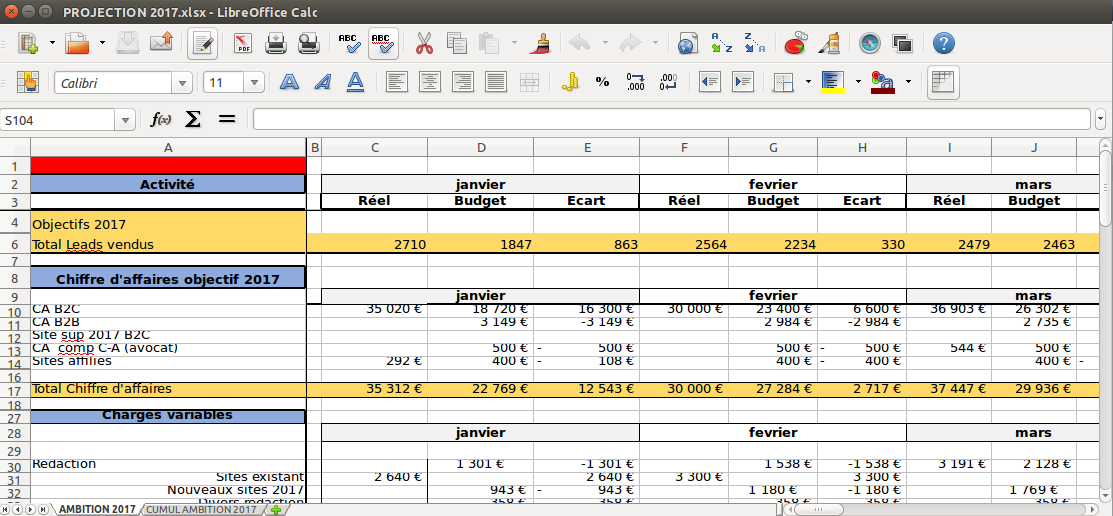
\includegraphics[width=300,height=250]{e1.png}}

\end{center}
\\








\subsection{ Spécifications fonctionnelles}


Le cahier des charges fonctionnel et technique est un document contractuel. Il résume le périmètre fonctionnel et technique du projet attendu par le client sur lequel le développeur s’engage de le réaliser.\\
La 2e section du cahier des charges consiste à rédiger les spécifications fonctionnelles et techniques du projet. C’est ici que j'ai  présenté en détail le dispositif du projet. \\

On va voir par la suite  des exemples où j'ai résumé quelques Spécifications fonctionnelles.

\subsubsection{L'accès au portail}
 
\begin{description}

\item[Fonctionnalité :] Page d'accueil.

\item[Description :] Une page d’accueil qui s'ouvre par
défaut en accédant au portail.

\item[Résultat :]  Tout utilisateur web peut accéder au site  par internet et visiter sa  page d'accueil qui contient le plan du portail et les informations de l'entreprise.

\end{description}


\subsubsection{ Création d’espace/entreprise}


\begin{description}

\item[Fonctionnalité :] Création de compte.

\item[Description :]  Un espace sécurisé et personnalisé permettant la gestion des données personnelles.

\item[Résultat :]  Toute entreprise client peut s'inscrire
au site de l'entreprise et avoir un compte dédié qui contient ses informations et ses données.

\end{description}

La création d'un espace Entreprise passe par les étapes suivantes:
\begin{itemize}


\item Demander à l'utilisateur d'entrer son adresse mail dans une zone de texte.
\item Demander à l'utilisateur d'entrer un pseudo dans une zone de texte.
Le pseudo devra contenir entre 3 et 25 caractères.
\item
Demander à l'utilisateur d'entrer un mot de passe qui devra compter entre 6 et 30 caractères, là encore dans une zone de
texte.
\item
Demander une confirmation du mot de passe.
Une fois les deux mots de passe entrés, si les deux mots de passe sont les
mêmes, on continue l'inscription.
Si ce n'est pas le cas, on redirige l'utilisateur vers une page d'erreur et on lui fait reprendre l'inscription du départ
\item
On l'envoie vers une seconde page de l'inscription, en le faisant cliquer sur un lien.

\end{itemize}



\subsubsection{Connexion}
\begin{description}


\item[Fonctionnalité :] Connexion .

\item[Description :]  accès au compte personnel par un pseudo et un mot de passe.

\item[Résultat :]  Chaque utilisateur peut accéder à
son espace personnel en toute sécurité.
\end{description}

\subsubsection{ Consultation des données}
\begin{description}

\item[Fonctionnalité :] Consultation .

\item[Description :]  Consulter les données et les informations du de l'entreprise.

\item[Résultat :]  Chaque utilisateur peut consulter toutes ses informations personnelles  et visualiser ses 
données.
\end{description}

\textbf{Consultation des indicateurs}:
\begin{itemize}
\item  Chiffre d’affaires
\item Couts
\item Marge
\item Résultat
\item Historiques
\end{itemize}


\subsubsection{ Importation/Exportation}
\begin{description}

\item[Fonctionnalité :] Importation/Exportation.

\item[Description :]  Importer et exporter des données et fichiers (xsl, csv )

\item[Résultat :]  l'utilisateur peut importer des fichiers Excel et télécharger les données sous forme
 des  fichiers csv.
\end{description}

\subsubsection{ Simulations }
\begin{description}

\item[Fonctionnalité :] Simulations.

\item[Description :]  permet de faire des hypothèses de projection de résultat.

\item[Résultat :]  Un tableau de bord interactif.
\end{description}

\subsubsection{Gestions des Editions}
\begin{itemize}

\item Compte de résultat 
 
\item Statistiques

\item Tableaux de bord
\end{itemize}

\subsubsection{Alert et Info}
\begin{description}

\item[Fonctionnalité :] Alert et Info.

\item[Description :]  Envoi des messages d'alertes et des e-mails d'informations aux utilisateurs.

\item[Résultat :]  En cas de création de compte, de changement de mot de passe et d'informations importantes, 
l'utilisateur reçoit des messages, à son adresse e-mail, de confirmation de versification et d'informations.
\end{description}



\newpage 

\section{ Choix techniques}


\subsection{Système d'exploitation}
Après la rédaction du cahier des charges  on passe à la recherches des solutions pour les besoins définis dans ce cahier. \\
A noter que j'avais toute la liberté de choisir, rien n'était exigé par l'entreprise, mais à condition que 
le choix soit bien justifié.\\ \\

Le système d'exploitation choisi est Linux avec sa distribution \textbf{Ubuntu 14.04} , il est open source, sécurisé et son environnement est bien adapté au développement du projet. 

\subsection{Architectures}
Un des plus célèbres design patterns s'appelle MVC, qui signifie Modèle - Vue - Contrôleur. C'est celui que je me suis basé pour la construction de l’architecture du site web.

Le pattern MVC permet de bien organiser son code source. Il permet de savoir quels fichiers créer, mais surtout à définir leur rôle. Le but de MVC est justement de séparer la logique du code en trois parties(Modèle - Vue - Contrôleur).\\

\begin{center}
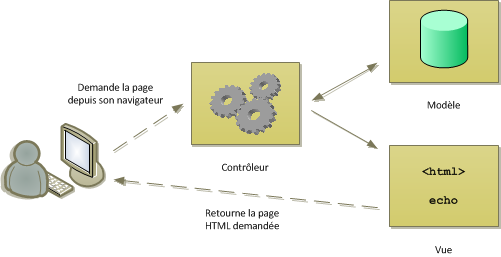
\includegraphics[width=300,height=250]{mvc.png}}

\end{center}


\subsection{Méthode de Programmation }

Les principales solutions existantes pour réaliser ce type de site Web sont :
\begin{itemize}
\item le codage « from scratch », c'est à dire en partant de zéro en utilisant un langage de programmation de A à Z.
\item l'utilisation d'un CMS qui  nous évite les lignes de codes .
\item l'utilisation d'un framework basée sur un langage de programmation.
\end{itemize} \\
La solution from scratch a été abandonnée, car elle est trop lourde et longue à
développer, surtout quand il s'agit d'un stage de quelques mois avec beaucoup des choses à réaliser.\\ 
Ainsi la solution CMS n'a pas été retenue puisqu'elle n'est pas adapté pour le genre de base de données interactive que 
je souhaite mettre en œuvre, avec la lenteur d'accès aux bases de données qui est visible surtout à l'affichage des pages
est un grand inconvénient d'un CMS.\\ \\

En revanche, l'utilisation d'un framework implique le développement sur-mesure de
tous les éléments du site à l'aide de fonctions relativement simples. L'apprentissage au
développement avec un framework apparaît plus simple qu'avec un CMS.\\

C'est pourquoi, le choix est d'utiliser un framework pour le développement du site web.\\

Mais le problème de choix ne s’arrête pas ici, il reste de préciser le choix du langage web et son framework.
 
\subsection{Langage web coté serveur }
Le langage de programmation utilisé va beaucoup influer sur le projet et la manière dont celui ci sera développé, en fonction des avantages et des inconvénients du langage.\\
On parle ici du langage back-end du site web, puisque le développement back-end est nécessaire pour bien gérer 
la bases de donnés, les  utilisateurs et les résultats à envoyer, en basant sur l'architecture MVC.\\ \\
Le choix du langage web est une autre étude qui a pris pas mal de temps en cherchant les différents langages, leurs  avantage et inconvénients. Les recherches étaient concentrés sur les langages suivants :
\begin{itemize}
\item PHP
\item Nodejs (JavaScript back-end)
\item Java (JavaEE)

\end{itemize}

Les autres langages ont été abandonné immédiatement par le motif de manque d'une base de connaissance permettant
l'apprentissage rapide du langage.\\ \\

Le choix du langage s’est finalement porté sur \textbf{PHP} avec sa version 5, qui 
 est un langage de script exécuté côté serveur. Langage qui permet une interaction avec l’utilisateur. Technologie permettant la création de pages web au contenu dynamique.\\

 En effet, il s’agit d’un langage facile
d’apprentissage, accessible sur la plupart des systèmes d’exploitations et très populaire sur le
web, ce qui permet un meilleur support et une meilleure maintenance. De plus, il s’agit d’un
langage déjà éprouvé depuis plusieurs années et donc assez robuste pour répondre aux
besoins de l’entreprise, qui veut s’appuyer sur des technologies matures et fiables pour
fonctionner de manière optimale. Enfin, il est assez facile d’apprentissage, ce qui permettra à
de futurs développeurs de maintenir ou de faire évoluer rapidement l’application.\\  \\




\subsection{Framework }
Un framework ou kit de développement est un espace de travail modulaire, c'est à dire
une suite d'outils et de bibliothèques qui facilitent et accélèrent le développement d'un
logiciel. Il contient toutes les fonctions de base utiles au développement d'un type de
programme, et permet donc de ne pas avoir besoin de réécrire les mêmes fonctions à
chaque programme créé. Il en existe dans tous les langages de programmation.\\ \\
J'ai testé et étudié les plus connus pour trouver le plus adapté:
\begin{itemize}
\item Symfony 3
\item Zend Framework 2
\item Laravel
\end{itemize} \\

 J'ai décidé d'utiliser Symfony 3 (précisément sa version 3.3), qui permet de  rendre le PHP beaucoup plus
confortable, l'AJAX plus abordable, l'optimisation du référencement (url rewriting) plus
simple.\\
Symphony est un Framework PHP qui a été lancé en 2005. Il est aujourd’hui stable et reconnu.
Il est également orienté objet, respecte le modèle MVC et est développé sous licence MIT.
C’est un Framework très utilisé et reconnu internationalement. Il a été développé par la société
SensioLabs qui l’utilise et le maintien régulièrement.
Il est considéré comme un ensemble d’outils rassemblant des composants préfabriqués,
rapides et faciles à utiliser.\\
Un des avantages de Symfony est de proposer une évolutivité et une maintenance efficace en
permettant à d’autres développeurs de prendre en main rapidement le projet sans avoir
participé à son élaboration. Il existe également un nombre important de ressources sur le web
pour rendre la maintenance encore plus facile. Enfin, il est très flexible car il permet de n’utiliser
que certains de ces modules sans forcément avoir à utiliser tout le Framework. Laravel
possède beaucoup de composants issus du Symfony.


\subsection{Bases de données}
 Le choix de la base de donnée  a prix beaucoup de temps de recherche et de comparaison entre les deux modèles
  \textbf{Relationnel} et \textbf{NoSql} représentés respectivement par \textbf{MySql} et \textbf{MongoDB}.\\
   \\
Et enfin j'ai choisi le modèle relationnel et son SGBDR MySql.\\

MySQL est le plus connu et utilisé des SGBD. Il repose sur le modèle relationnel, des tables ont des enregistrements , et ces tables peuvent avoir des relations.\\  Ceci a l’avantage de pouvoir lier très facilement des enregistrements d’une table à l’autre.\\  De plus, lors des enregistrements, les transactions sont soumises aux contraintes ACID (atomicité, cohérence, isolation et durabilité), ce qui signifie qu’un enregistrement incomplet ou incorrect ne sera pas enregistré en base. \\  MySQL permet ainsi de facilement structurer les informations et de les réutiliser avec aisance. Finalement, MySQL est un système où l’intégrité des enregistrements est pris en charge par le logiciel et le risque d’erreurs est donc peu élevé.


  
   

\subsection{Langages web coté client}

L'effet de choisir ce n'est pas toujours simple surtout dans le cas où les concurrents sont très proches.
Mais heureusement dans la parie font-end (coté client) les choses sont claires et il n'y a quasi pas de choix.

L'utilisation des langages suivants est nécessaire et parfois est indispensable  :
\begin{itemize}
\item \textbf{HTML5:} L’Hypertext Markup Language(HTML), est le format de données conçu pour gérer
et organiser le contenu d'une page web. C’est un langage de balisage qui
permet d’écrire de l’hypertexte, d’où son nom. C'est un langage de description
de données, et non un langage de programmation. Je l’ai utilisé pour créer la
partie statique du site web.

\item \textbf{CSS3:} Cascading Style Sheets : feuilles de style en cascade est un langage informatique
qui sert à décrire la présentation des documents HTML (et XML). Les standards
définissant les CSS sont publiés par le World Wide Web Consortium (W3C). Introduit au
milieu des années 1990, le CSS devient couramment utilisé dans la conception de sites
web et bien pris en charge par les navigateurs web.

\item \textbf{JAVASCRIPT:} Javascript est un langage de programmation de type script, non compilé, orienté
objet, principalement utilisé dans les pages Web. C’est un langage exécuté  côté client, c'est-à-dire par le navigateur de l’utilisateur. Il a pour but de dynamiser les
sites Internet.
\end{itemize}

\subsection{Technologies et Outils}

On peut résumer la suite  des frameworks et des  bibliothèques utilisés  par la liste suivante :
\begin{itemize}

\item \textbf{JQUERY:} En JavaScript j’ai utilisé plus particulièrement ​
jQuery, qui est une bibliothèque
JavaScript libre qui porte sur l'interaction entre JavaScript
(comprenant Ajax) et HTML, et a pour but de simplifier des
commandes communes de JavaScript. C’est avec cette technologie que j’ai réalisé la partie dynamique coté client du site web.

\item \textbf{AJAX:} AJAX est l'acronyme d'Asynchronous JavaScript And XML, autrement dit JavaScript Et XML Asynchrones.
L'idée  est de faire communiquer une page Web avec un serveur Web sans occasionner le rechargement de la page. 

\item \textbf{BOOSTRAP:} kit CSS créé par les développeurs de Twitter, est devenu en peu de temps le framework CSS de référence. Il permet de  construire rapidement et facilement des sites web esthétiques et responsives. Bootstrap offre aussi des plugins jQuery de qualité pour enrichir les pages.

\item \textbf{WEBSOCKET:} WebSocket est une alternative à Ajax plus simple à mettre en oeuvre coté client, mais avec une compatibilité limitée aux navigateurs récents.

\item \textbf{TWIG:} Dans Symfony le PHP et le HTML sont entièrement séparer, le HTML est inséré
dans les fichiers Twig. Twig est un moteur de template PHP
directement intégré dans Symfony3 et créé lui aussi par Sensio. Très
puissant, Twig permettra de gérer de l’héritage entre templates et
layout, séparer les couches de présentation et couche métiers.

\item \textbf{Doctrine: } l'ORM par défaut de Symfony. L'objectif d'un ORM (pour Object-Relation Mapper, soit en français « lien objet-relation ») est simple : se charger de l'enregistrement des données en  faisant oublier qu'il n'y a pas  une base de données.

\end{itemize}
\\ 
\\

\subsubsection{Outils}

\begin{itemize}


\item \textbf{GIT:} un outil qui va  permettre de versionner le code source, c'est-à-dire gérer les versions du code au fur et à mesure. j'ai l'utilisé pour pour héberger le code source  en github, en cas de panne locale le
code est facile à récupérer.

\item  \textbf{Apache2:} est un serveur HTTP créé et maintenu au sein de la fondation Apache. C'est le serveur HTTP le plus populaire du World Wide Web. il me permet de tester le site localement.

\item  \textbf{Netbeans:} est un environnement de développement intégré (EDI) open source. Il a
été créé par Sun en juin 2000. NetBeans permet de supporter de nombreux
langages dont PHP, HTML, Twig, Javascript et YML. C’est sous cet environnement que j’ai programmé l’intégralité du portail.


\item \textbf{draw.io:} c'est un outil en ligne permettant de faire des design des maquettes, templates et l’architecture du site web.

\item \textbf{Umbrello:} c'est un logiciel linux open source permettant de faire des diagrammes UML.

\item \textbf{Mysql-server:} le serveur de la base de données MySql

\item \textbf{PhpMyAdmin: } Permettant de visualiser le données au navigateur.

\item \textbf{FileZila:} Transfert ftp.

\item \textbf{TexMaker} Éditeur latex pour la rédaction du cahier de charges, des comptes rendu et des rapports.
\end{itemize}



\newpage

\section{Conception et Modélisation  }

\subsection{Conception}

Dans la phase d’analyse, le diagramme de classes représente les entités (des informations) manipulées par les utilisateurs.\\
Dans la phase de conception, il représente la structure objet d’un développement orienté objet.\\
\\

\begin{center}
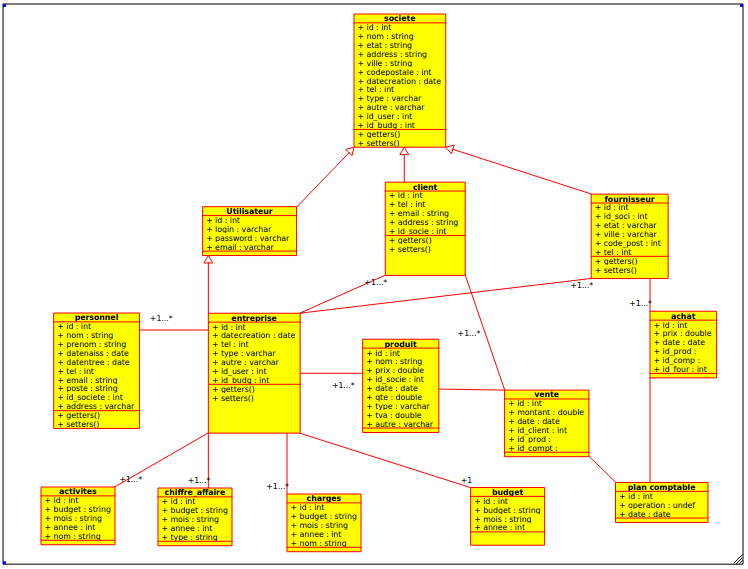
\includegraphics[width=300,height=250]{dc.png}}

\end{center}



Pour simplifier les choses, on peut résumer les principales fonctionnalités, déjà précisés dans le cahier des charges, par un diagramme UML de cas d'utilisation , qui  représente les fonctionnalités (ou dit cas d’utilisation) nécessaires aux utilisateurs. On peut faire un diagramme de cas d’utilisation pour quelques 
fonctionnalité du site web. 

\\
\\

\begin{center}
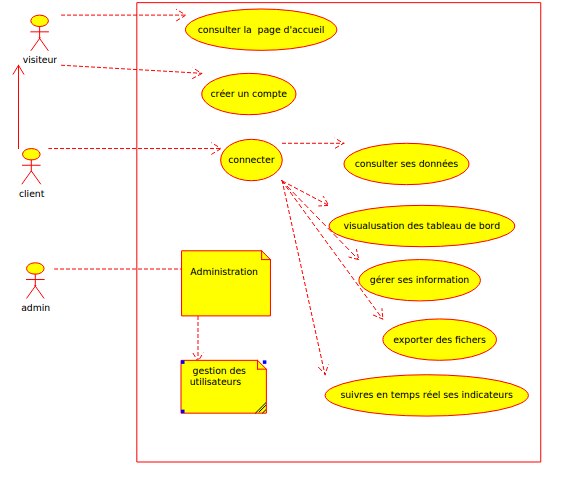
\includegraphics[width=300,height=250]{cd2.png}}

\end{center}


\\
\\

Toutes les fonctionnalités détaillées dans le cahier des charges, devront être dans les bonnes places de l'interface web du site internet.\\
Ainsi j'ai procédé par la suite à modéliser l'ensemble des pages du portail afin de mettre chaque 
fonctionnalité à sa place.\\




\begin{center}
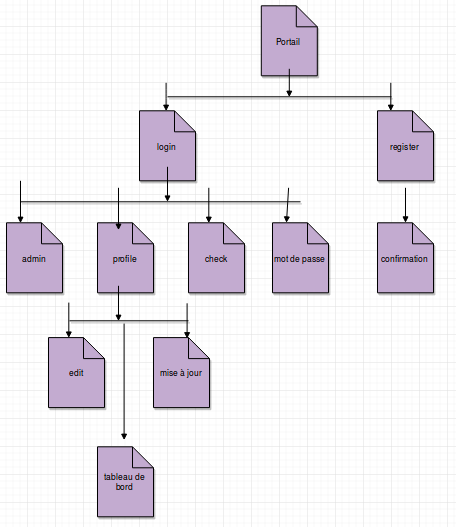
\includegraphics[width=300,height=250]{p3.png}}

\end{center}

\\ \\
J'ai choisi de minimiser le nombre des pages et des routes , en utilisant des pages
\textbf{scrolling} qui contiennent plusieurs sections.







\subsection{Modélisation}
\subsubsection{Modélisations des données}


Une base de données relationnelle s'appuie sur un modèle relationnel et donc il s'agit d'un système possédant des relations entre ses différentes parties .\\ \\

La modélisation de la base de données est également une tâche très importante car il s’agit
du cœur du site web réalisée. \\ 


\\ \\

\begin{center}
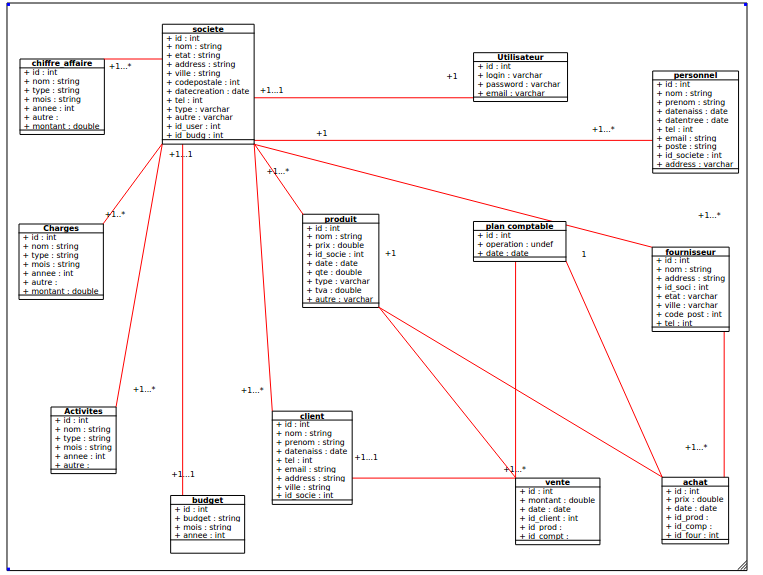
\includegraphics[width=300,height=250]{bd1.png}}

\end{center}
\\ \\

La figure ci-dessus représente la base de données réalisée, à noter que toutes les attributs des entités  ne s'affichent pas dans la figure .\\ Nous pouvons constater que quasiment toutes les tables sont reliées à la table « societe » . Cela nous indique que les requêtes effectuées sur la base de données concernent essentiellement les sociétés, qui sont les clients de \textbf{VMP-CONSULTING}.\\
La base de données elle-même comportant un nombre assez important de tables.\\
Ces tables sont  très complètes avec une grande quantité d’attributs. Il est possible que
ces attributs soient trop nombreux et doivent être séparés pour être mis dans des nouvelles
tables.\\



\subsubsection{Maquette et Responsive design}

Une maquette permet de vérifier avec le client tous les aspects visuels du site, de la mise en page générale aux détails tels que les couleurs, les polices , les images, les icônes, les logos… etc.\\
Elle est l’équivalent du site web en version imprimée. La création de la maquette vient suite à l’étude des besoins du client et l’élaboration d’un cahier des charges.\\

 \\
\\


\begin{center}
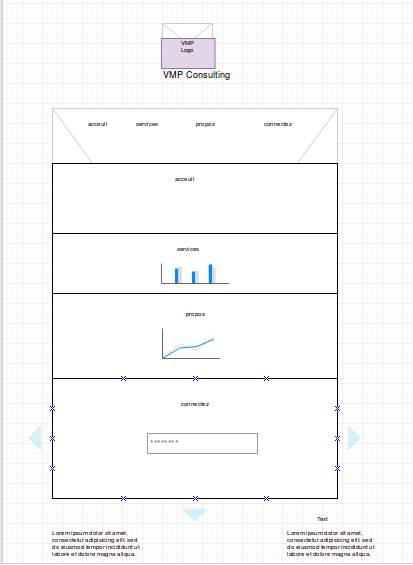
\includegraphics[width=300,height=250]{mod2.png}}

\end{center}

\\ \\


Le responsive design est vraiment incontournable dans le processus de création d’un site web.  C'est parce que internet est maintenant présent sur tous les écrans, que ce n'est plus possible de concevoir un site web sans penser au responsive design.\\
Un temps de conception d'une maquette responsive est nécessaire afin d'avoir une vision globale et précise de site responsive.\\ \\
Le responsive design est une fonctionnalité importante du cahier des charges.
Et la  de la maquette ci-dessus  a été traduite en \textbf{html5} et \textbf{CSS3}, pour devenir une  interface web responsive
 à l'aide de \textbf{Boostrap}.\\
Cette interface a été  dynamisé par \textbf{javascript} et sa librairie \textbf{JQuery}.
 
 \\
 \\

\begin{center}
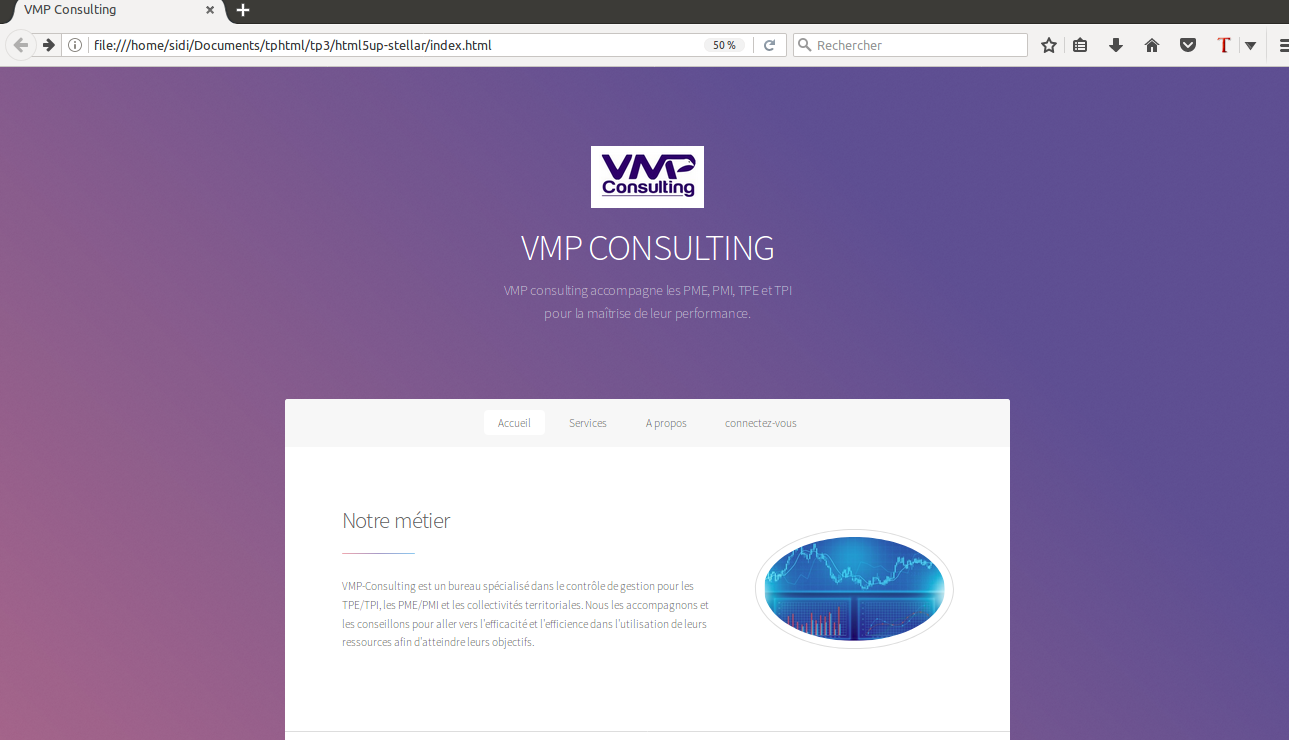
\includegraphics[width=300,height=250]{design1.png}}

\end{center}

\\ \\ 


\newpage

\section{Développement et Implémentation}

\subsection{Installation et Configurations}


Symfony est le Framework PHP utilisé, crée par SensioLabs basé sur une
architecture MVC( Modéle, vue et contrôleur ). Ce framework a été choisi
en raison des motifs expliqués dans la partie \textbf{Framework}.\\
La version utilisé est la dernière version sortie à l’écriture de ce rapport \textbf{symfony 3.3}.
\\

\subsection{La Base de Donnés Relationnelle }

\subsection{Administration}

\subsection{Tableau de bord}

\subsection{Sécurité}

\subsection{Temps réel}

\subsection{Services}



\newpage

\section{Test}

\subsection{Démonstrations}

\begin{center}

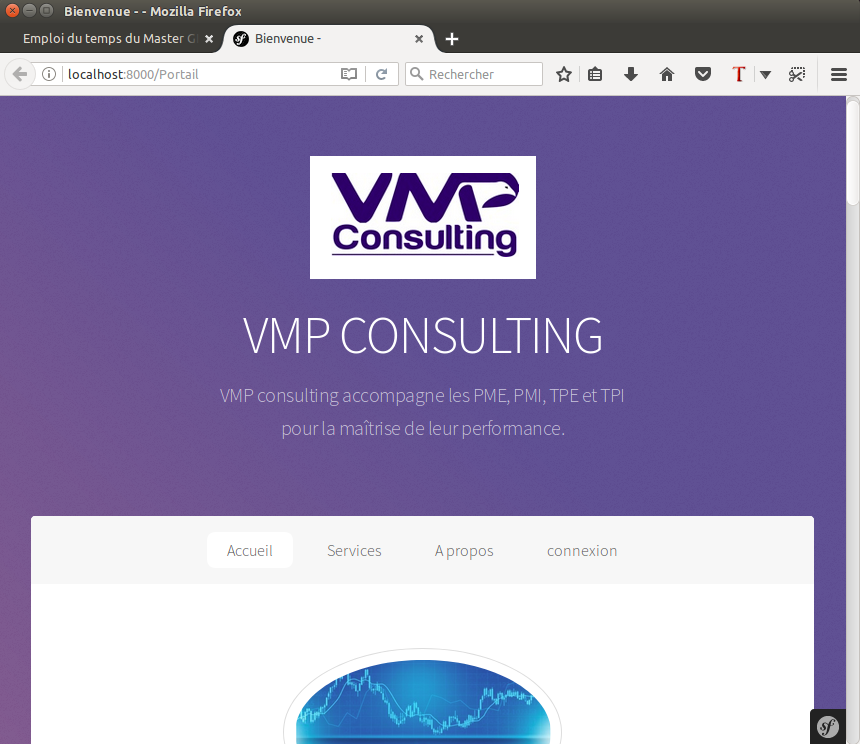
\includegraphics[width=300,height=250]{v1.png}} \\ \\
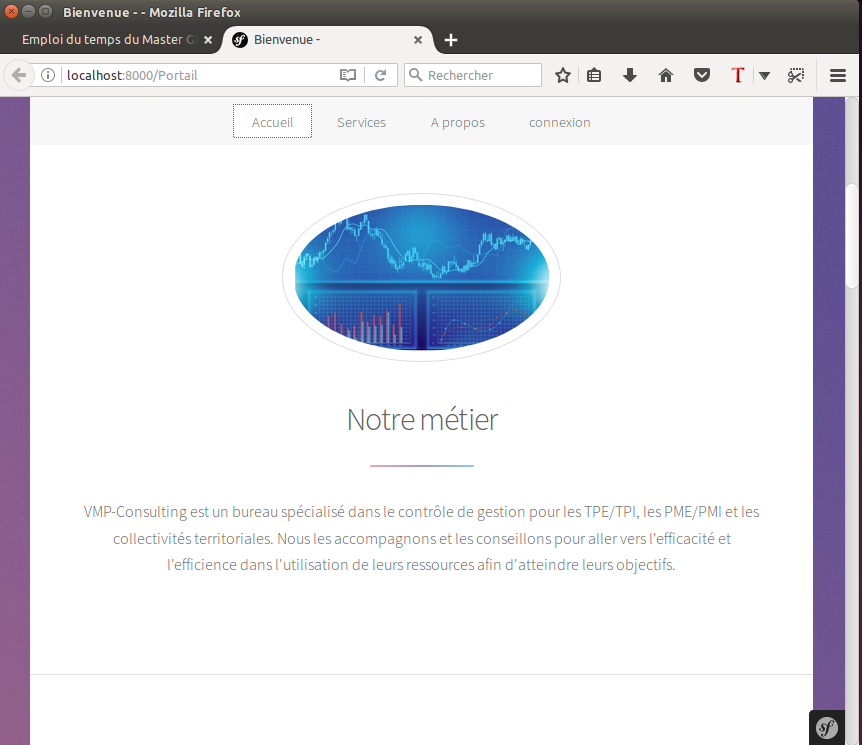
\includegraphics[width=300,height=250]{v2.png}} \\ \\
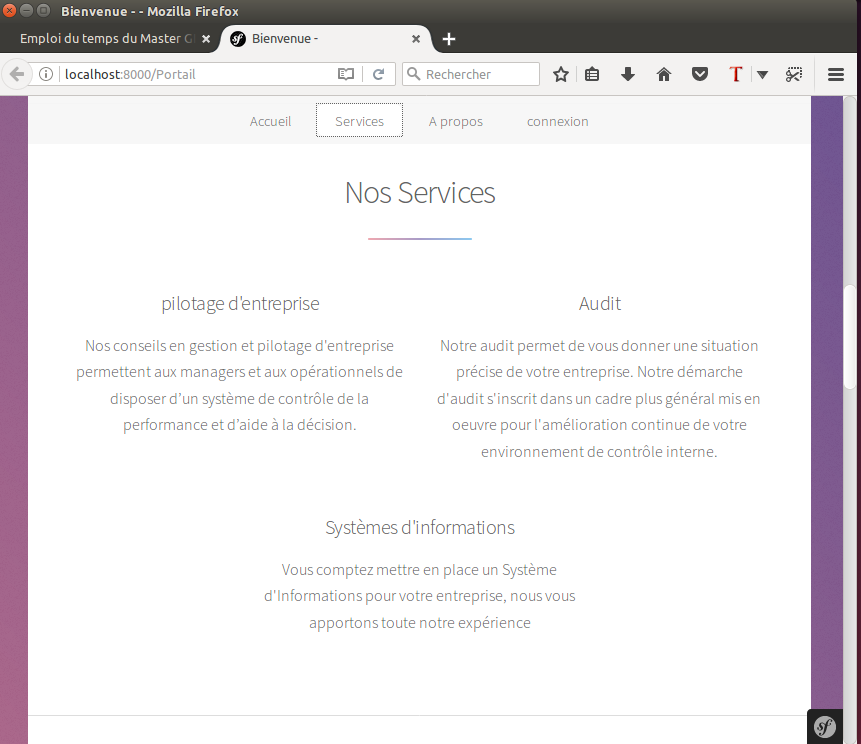
\includegraphics[width=300,height=250]{v3.png}} \\ \\
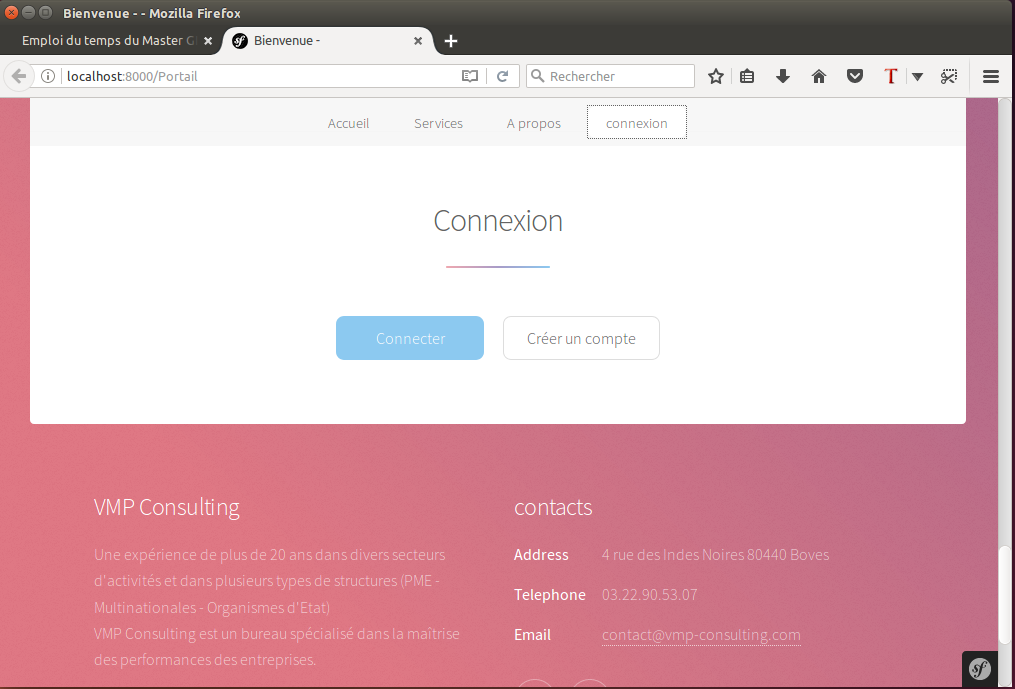
\includegraphics[width=300,height=250]{v4.png}} \\ \\
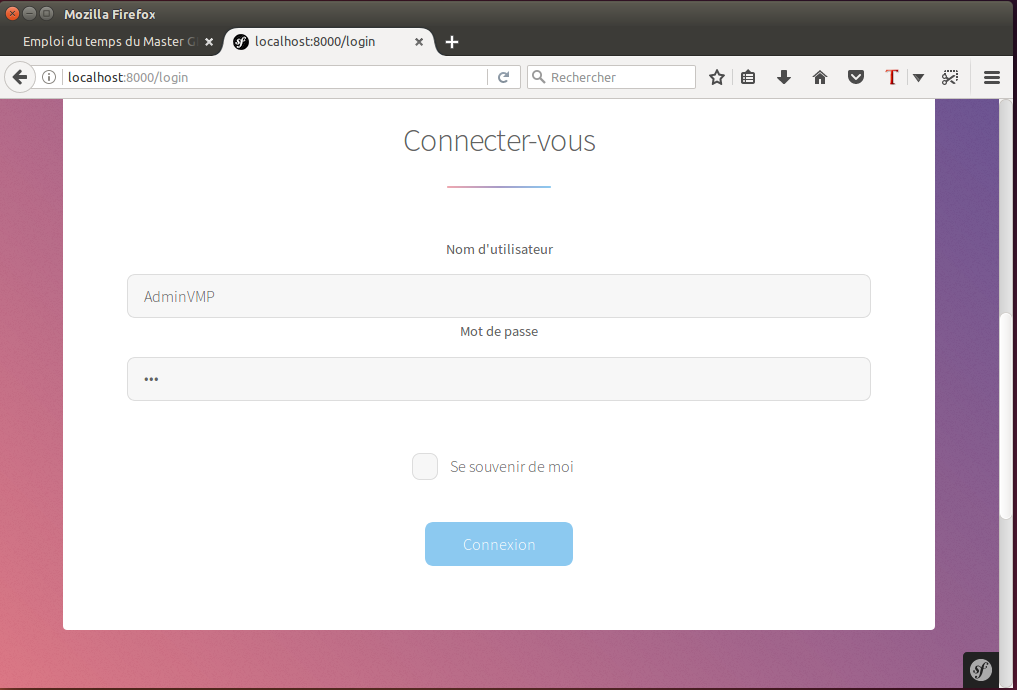
\includegraphics[width=300,height=250]{v5.png}} \\ \\
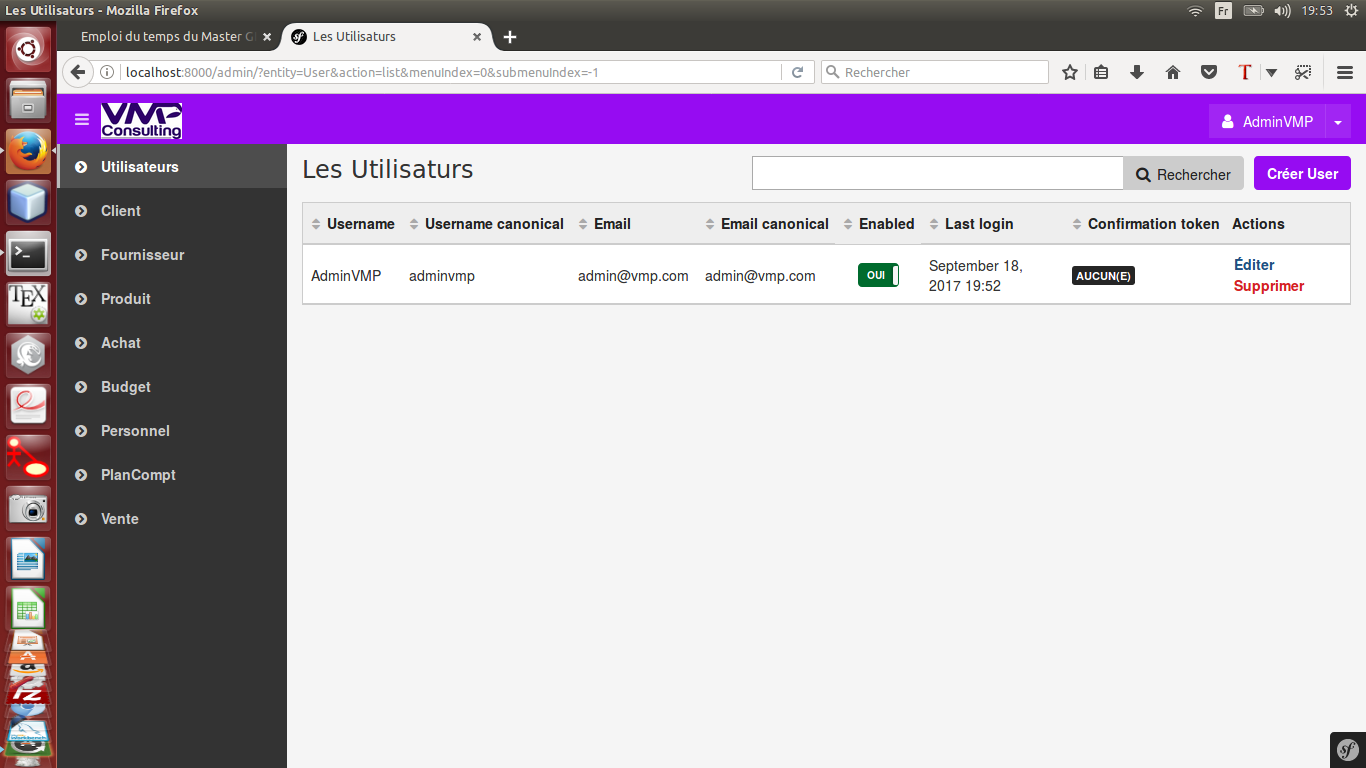
\includegraphics[width=300,height=250]{v6.png}} \\ \\
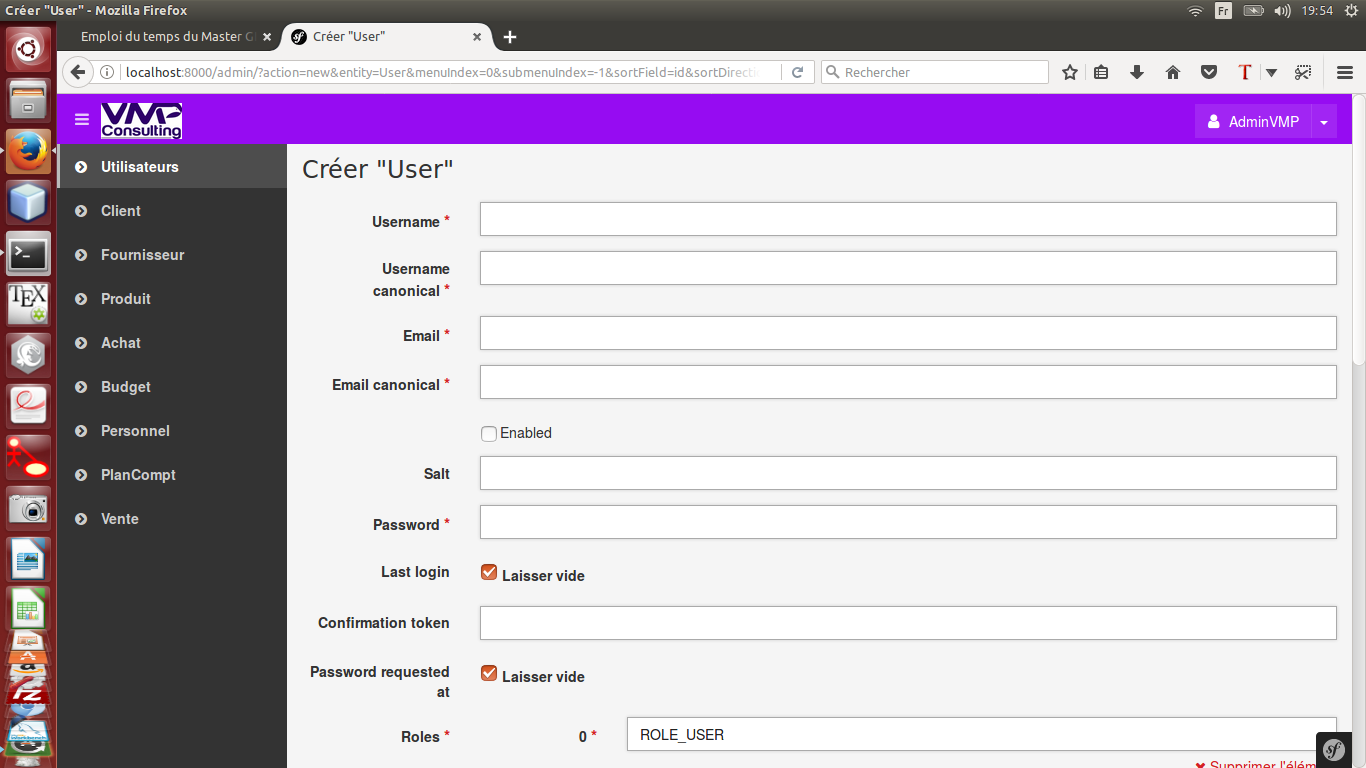
\includegraphics[width=300,height=250]{v7.png}} \\ \\
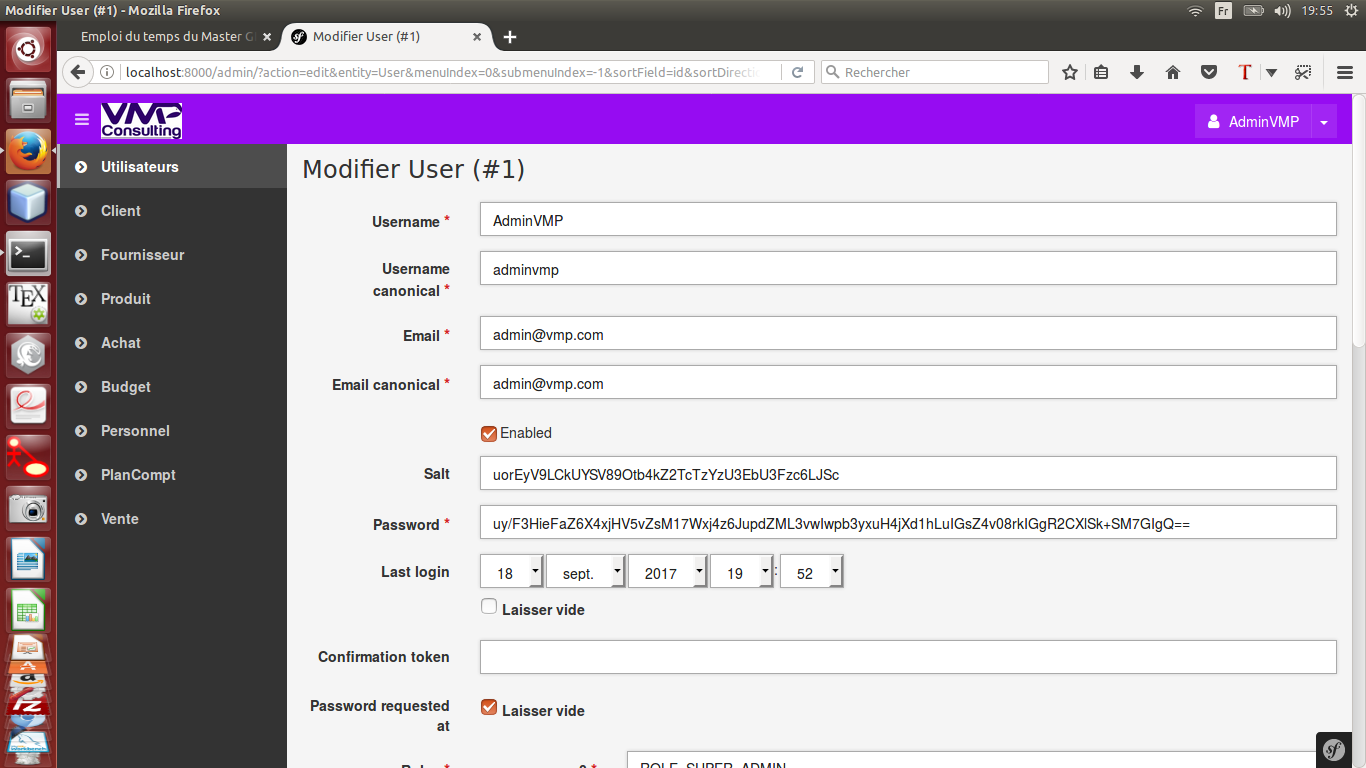
\includegraphics[width=300,height=250]{v8.png}} \\ \\
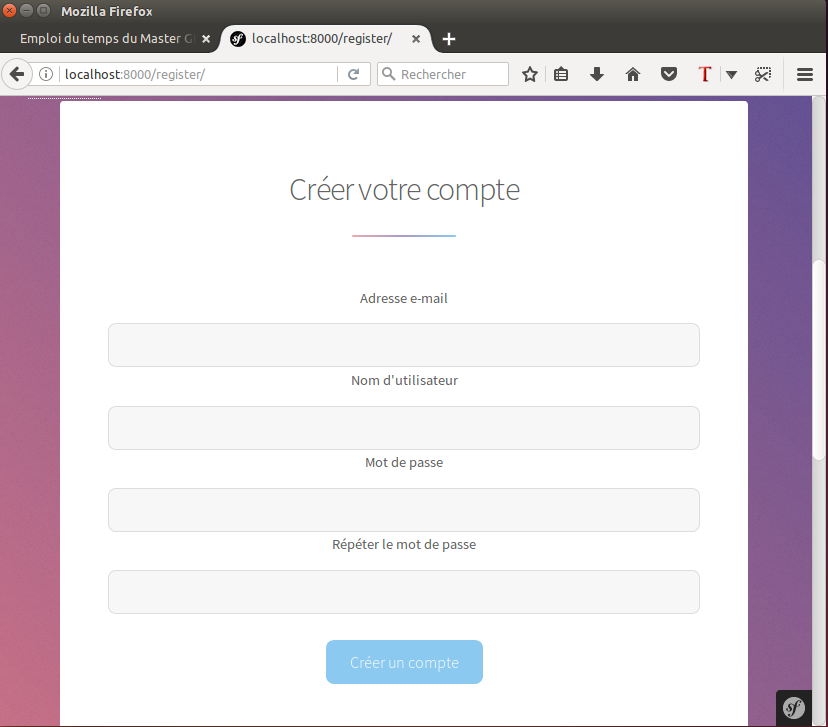
\includegraphics[width=300,height=250]{v9.png}} \\ \\
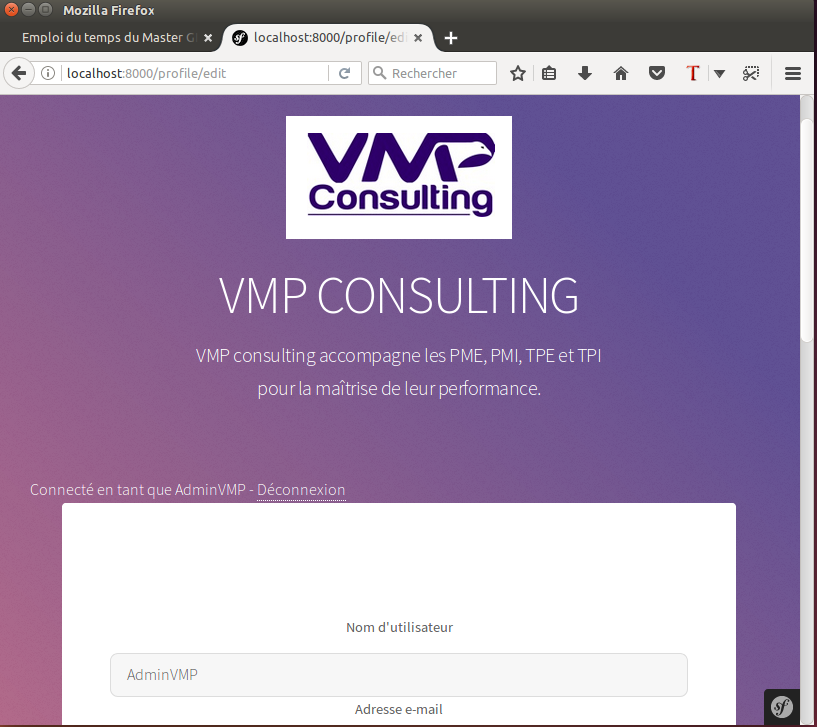
\includegraphics[width=300,height=250]{v10.png}} \\ \\

\end{center}

\subsection{Bilan}



\newpage
\section{Conclusion}


\newpage
\section{Bibliographie}


\end{document}
